\chapter{Données d'évaluation des trous noirs}
\label{ch-a}

\begin{figure}[h]
    \begin{subfigure}[t]{.45\linewidth}
        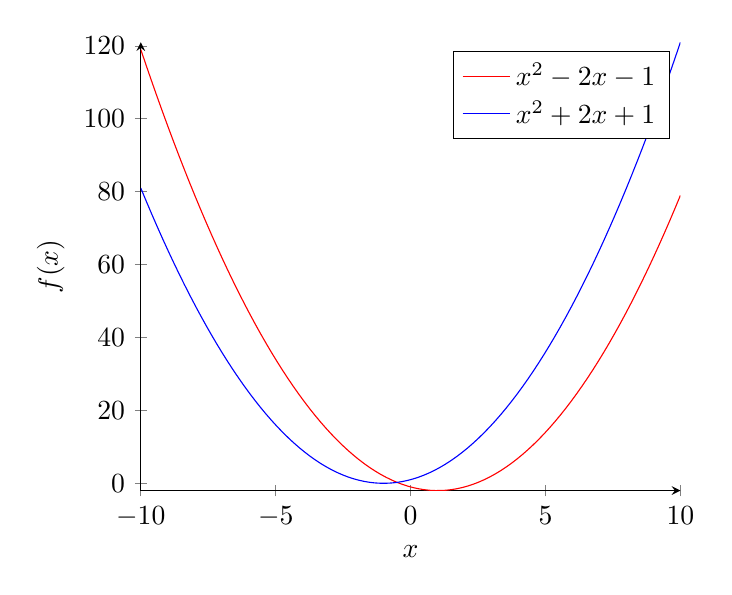
\begin{tikzpicture}
    \begin{axis}[
            axis lines = left,
            xlabel = \(x\),
            ylabel = {\(f(x)\)},
        ]
        \addplot [
            domain=-10:10,
            samples=100,
            color=red,
        ]
        {x^2 - 2*x - 1};
        \addlegendentry{\(x^2 - 2x - 1\)}
        \addplot [
            domain=-10:10,
            samples=100,
            color=blue,
        ]
        {x^2 + 2*x + 1};
        \addlegendentry{\(x^2 + 2x + 1\)}
    \end{axis}
\end{tikzpicture}
        \caption{Example de graphique de fonctions.}
        \label{fig-graphique}
    \end{subfigure}
    \hfill
    \begin{subfigure}[t]{.45\linewidth}
        \begin{tikzpicture}
    \begin{semilogxaxis}[
            xlabel=magnitude apparente $V$, % Set the labels
            ylabel=distance,
            x unit=, % Set the respective units
            y unit=al,
            x tick label style={rotate=90,anchor=east}
        ]
        \addplot table[x=Magnitude,y=Distance,col sep=comma]{figures/appendixA/data.csv};
    \end{semilogxaxis}
\end{tikzpicture}

        \caption[Autre exemple de graphique.]{Autre example de graphique généré à partir du fichier \texttt{figures/appendixA/data.csv}.}
        \label{fig-graphique-csv}
    \end{subfigure}
    \caption{Cette fois-ci, aucun \gls{trou_noir}.}
\end{figure}

Les \cref{fig-graphique,fig-graphique-csv} sont des exemples créés à l'aide de la bibliothèque PGFPlots.


\begin{longtable}{lllS[table-format=3.2]S[table-format=3.5]}
    \toprule
    nom  & désignation de  Bayer & type spectral & {magnitude}  & {distance (al)} \\ \midrule
    \csvreader[head to column names,separator=comma,late after line=\\,late after last line=\\\bottomrule]{figures/appendixA/data.csv}{}{\Nom&\Bayer&\Type&\Magnitude&\Distance}
    \caption{Tableaux des données utilisées par \ref{fig-graphique-csv}.}
\end{longtable}

% Other example with pgfplotstabletypeset?

% \pgfplotstabletypeset[
%     begin table=\begin{longtable},
%     every first row/.append style={before row={%
%         \caption{Tableaux des données utilisées par \ref{fig-graphique-csv}.}%
%         \endfirsthead
%         \multicolumn{3}{c}{{\bfseries \tablename\\
%         \thetable{} -- suite}} \\
%         \endhead
%     }},
%     columns={Nom,Bayer,Type,Magnitude,Distance},
%     every head row/.style={before row=\toprule,after row=\midrule},
%     every last row/.style={after row=\bottomrule},
%     columns/Nom/.style={string type},
%     columns/Bayer/.style={string type,column name={désignation de Bayer}},
%     columns/Type/.style={string type},
%     % columns/Magnitude/.style{string type,column type={S[table-format=1.2]}},
%     % columns/Distance/.style{string type,column type={S[table-format=3.5]}},
%     col sep=comma,
%     end table=\end{longtable}
% ]{figures/appendixA/data.csv}